%% Begin:
%% mode: xelatex
%% End:

% Run
% xelatex "\def\ishandout{1} \documentclass[a4paper]{article}

\usepackage{fontspec}
\usepackage[brazil]{babel}
\usepackage{a4wide}
\usepackage{tikz}
\usetikzlibrary{automata,circuits,matrix,shapes.gates.logic.US,positioning}
\usepackage{circuitikz}

%%%%%%%%%%%%%%%%%%%%%%%%%%%%%%%% DEFS
\newcounter{exc}
\def\exercise{\bigskip
  \addtocounter{exc}{1}{\bf Exercício \arabic{exc}.}}
\def\set#1{\{#1\}}
\def\<#1>{\langle#1\rangle}
\def\tuple#1{{\langle #1\rangle}}%
\def\topic#1{\bigskip{\bf #1}}
\def\lcompl#1{\overline{#1}} % logical complement
\def\lxor{\oplus}

% image directory
\def\imgdir{../_img}

\title{Introdução a Sistemas Digitais}
\author{Adriano J. Holanda}
\date{\today}

%%%%%%%%%%%%%%%%%%%%%%%%%%%%%

\begin{document}
\maketitle

\input bool

\input sequential-circuits

\end{document}
"
% to disable transitions

\ifdefined\ishandout
  \documentclass[notheorems,handout]{beamer}
\else
  \documentclass[notheorems]{beamer}
\fi

\setbeamercovered{highly dynamic}
\newcounter{saveenumi}% save counter on enumerate across frames
\newcommand{\seti}{\setcounter{saveenumi}{\value{enumi}}}
\newcommand{\conti}{\setcounter{enumi}{\value{saveenumi}}}
\resetcounteronoverlays{saveenumi}

% Dependencies
\usepackage{fontspec} % use XeLaTeX
\usepackage[]{polyglossia}
\setdefaultlanguage{brazil}
% \usepackage{lcg} % Generate random numbers
\usepackage{hyperref}
\hypersetup{colorlinks=true,linkcolor=blue,anchorcolor=blue,urlcolor=blue}
\usepackage{pgf,tikz} % Draw figures
\usetikzlibrary{arrows,automata,calc,chains,circuits,graphs,positioning,shapes.gates.logic.US,shapes,trees}
\usepackage{circuitikz}
%\usepackage{pgfgantt}
  % \usepackage{pgfplots}
  % \usegdlibrary{trees}
  \usepackage{listings}
  \lstset{language=C,inputencoding=utf8,basicstyle=\footnotesize, 
    flexiblecolumns=true, numbers=left, numberstyle=\tiny\color{gray}, 
    commentstyle=\scriptsize\color{black!50},mathescape}
  \usepackage{pdftexcmds} % \pdf@strcmp \pdf@filemoddate
  \usepackage{ifthen} % \ifthenelse
  \usepackage{animate}

  % FONTS
  \font\fiverm=cmr5
  \font\ninerm=cmr9

  % Definitions
  \author{Adriano J. Holanda}%\\{\scriptsize \url{http://holanda.xyz}}}
  \def\array{vetor}
  \def\bigO#1{\mathcal{O}(#1)}
  \def\bug#1{{\it bug#1\/}}
  % C letter
  \font\ninerm=cmr9
  \let\mc=\ninerm
  \def\CEE{{\mc C\spacefactor1000}}

  \def\boxset{
    \tikzset{box/.style={rectangle,minimum width=.5cm,draw},
      index/.style={minimum width=.5cm}}
  }

  % only title frames
  \def\onlytitleframe#1{\author{}\date{}\title{#1}\maketitle}

  % THEOREM
  % \newtheorem{teorema}[theorem]{Teorema}

  \newcommand{\executeiffilenewer}[3]{%
    \ifnum\pdf@strcmp{\pdf@filemoddate{#1}}%
    {\pdf@filemoddate{#2}}>0%
    {\immediate\write18{#3}}\fi%
  }
  % includesvg[includegraphics args]{file} command (linux-version)
  \newcommand{\includesvg}[2][]{%
    \executeiffilenewer{#2.svg}{#2.pdf}{%
      /usr/bin/inkscape -z -C --file="#2.svg" --export-pdf="#2.pdf" > /tmp/#2.log}%
    \ifthenelse{\equal{#1}{}}{%
      \includegraphics{#2}}{%
      \includegraphics[#1]{#2}}%
  }

\def\lecturetitle#1#2{\title{{\large\bf#1}\\{\small [#2]}}}

\def\transitionslide#1{\frame{\author{}\title{\LARGE#1}\date{}\maketitle}}

  \def\shcmd#1{
    \begingroup
    \bigskip\color{gray}
    {\tt \$~#1}
    \bigskip
    \endgroup
  }


  \def\fonte#1{\begingroup\tiny\tt\color{gray} Fonte:~#1\endgroup}

\usetikzlibrary{automata,matrix,positioning,shadows,shapes,shapes.geometric,topaths,backgrounds,shapes.callouts}

\newtheorem{theorem}{Teorema}
\newtheorem{lemma}[theorem]{Lema}
\newtheorem{corollary}[theorem]{Corolário}
\newtheorem{definition}[theorem]{Defini\c{c}\~ao}

\def\imgdir{../_img/}

\def\course{Introdução à Organização de Computadores}

%%%%%%%%%%%%%%%%%%%%%%%%%%%%%%%% DEFINES
\def\AXIOM{{\color{gray}\tt\scriptsize [axioma]}}
\def\THEOREM{{\color{gray}\tt\scriptsize [teorema]}}
\def\NOT#1{{\overline{#1}}}

\def\dec#1{$#1_{10}$}

\def\side{3cm}
\def\flabel#1{\scriptsize{#1}}

\def\framefigtanenbaum{
  \begin{frame}[label=fig:tanenbaum]
    \frametitle{Organização de um computador simples\footnote{\tiny Figura adaptada de Tanenbaum,2007, pg 29.}}
    
    \def\side{3cm}
\def\flabel#1{\scriptsize{#1}}
   \begin{tikzpicture}

   \tikzset{scale=0.8,
     boxtext/.style={text width=2cm,text centered, midway}}

     %CPU
     \draw (0,0) rectangle +(\side,\side);
     \foreach \x / \y in {1/1,2.25/1,1/2,2.25/2} {
       \def\factor{0.25*\side}
       \draw (\factor*\x,\factor*\y) rectangle +(0.2*\side,0.1*\side);
       % draw vertical dots
       \ifnum\y=1%
       \node at (\factor*\x+0.1*\side,\factor*\y+0.22*\side) {$\vdots$};
       \fi
     }
     \node at (0.5*\side,0.75*\side) {\flabel{Registradores}};
     \draw (0,1.1*\side) rectangle +(\side,0.6*\side) 
     node[boxtext] {\flabel{Unidade l\'ogica e aritm\'etica (ALU)}};
     \draw (0,1.8*\side) rectangle +(\side,0.5*\side) 
     node[boxtext] {\flabel{Unidade de controle}};
     % cpu
     \draw (-0.25cm,-0.5cm) rectangle +(0.475cm+\side,2.6*\side)
     node[above] {\flabel{Unidade central de processamento (CPU)}};

     % dev
     \draw (1.2*\side,0) rectangle +(0.75*\side,0.5*\side) 
     node[boxtext] {\flabel{Mem\'oria principal}};

     % I/O
     \draw (0.25cm+2*\side,0) rectangle +(0.75*\side,0.5*\side) 
     node[boxtext] {\flabel{Disco}};
     \draw (3*\side,0) rectangle +(0.75*\side,0.5*\side) 
     node[boxtext] {\flabel{Impressora}};
     % I/O label
     \draw[|-|] (0.2cm+2*\side,0.55*\side) -- +(1.7*\side,0) 
     node[midway,above] {{\tiny Dispositivos de E/S}};


     % bus startx at cpu box
     \draw[draw=red,very thick] (0.5*\side,-0.5cm) to (0.5*\side,-1cm)
     to (1.55*\side,-1cm) to (1.55*\side,0)
     to (1.55*\side,-1cm) to (0.25cm+2.35*\side,-1cm)
     to (0.25cm+2.35*\side,0) to (0.25cm+2.35*\side,-1cm)
     to (3.35*\side,-1cm) to (3.35*\side,0)
     to (3.35*\side,-1cm) to (4.35*\side,-1cm) node[above] {\flabel{Barramento}};

     %% becomes noise
     %%\node[text width=3cm] at (4*\side,1.75*\side) {\flabel{1 CPU + 2 dispositivos de entrada e saída}};
\end{tikzpicture}

  \end{frame}

} % end  framefigtanenbaum


\def\framevonneumannarch{
\begin{frame}
  \frametitle{``Máquina'' de von Neumann}
  
% draw of von Neumann machine
\usetikzlibrary{shapes.arrows}
\def\height{1.75cm}
\def\width{2.5cm}
\begin{tikzpicture}[scale=0.9,
  module/.style={anchor=west,draw,rectangle,minimum width=\width,minimum height=\height},
  vdarrow/.style={anchor=west,double arrow,draw=blue,fill=blue!30,minimum height=1.25cm}, % vertical double arrow
  hdarrow/.style={vdarrow,rotate=90} % horizontal double arrow
  ]
  \node[name=a,module] at (0,0) {Aritm\'etica};
  \node[name=ac,vdarrow,shift=(a.east)] {};
  \node[name=c,module,shift=(ac.east)] {Controle};
  \node[name=ces,vdarrow,shift=(c.east)] {};
  \node[name=es,module,shift=(ces.east)] (es) at (2*\height+2*\width,0) {E/S};
  % ATENTION HERE: rotating the double arrow dont change
  % the position names, so east continues being the extremity
  \node[name=ces,hdarrow,shift=(c.north)] {};
  \node[name=mem,module,anchor=south,shift=(ces.east)] {Mem\'oria};
  \draw[dashed,draw=red] (-0.5,-1.65) node[below right]
  {\color{red}{\scriptsize{Unidade central}}} rectangle (7.75,1.65);
\end{tikzpicture}

\end{frame}
}

\def\framemipsprocfigure{
\begin{frame}{Estudo de caso -- processador MIPS32 M4K\footnote{\tiny Reproduzido com
      permissão da \href{http://www.mips.com/}{MIPS Technologies}.}}

  {\tiny MDU -- unidade de multiplicação/divisão\hspace{1cm}
    MMU -- unidade de gerenciamento de memória \\
    SRAM -- memória de acesso aleatório estática}  
  
\begin{center}
  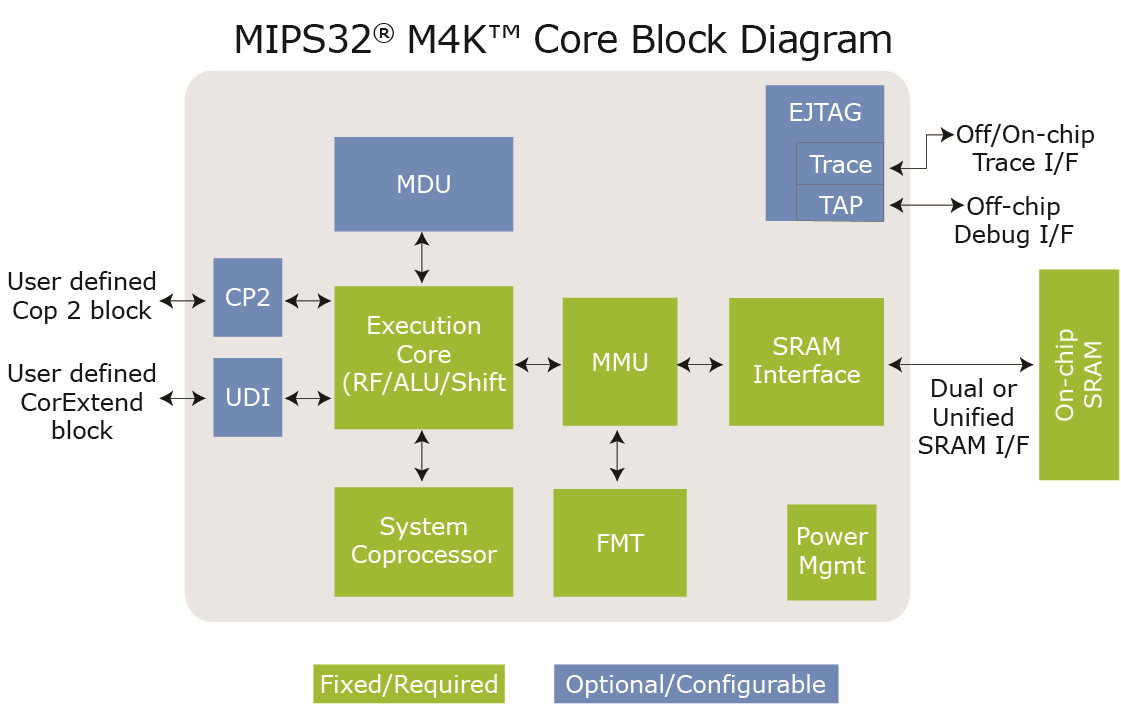
\includegraphics[scale=.25]{\imgdir/M4KcoreBlockDiagram.png}
\end{center}

\end{frame}
}

% References with ISBN
\def\tocciref{Sistemas Digitais. Tocci;
      Widmer \& Moss. 
\href{http://www.pearson.com.br/produtos_detalhes.asp?id_p=0&livro_cod=9788576059226&pag_id=3&area_pai=21}{ISBN-13:
        978-85-7605-922-6}}

\usecolortheme{crane}

%\includeonlylecture{proc}

\begin{document}
\date{\today}

\input history

\input representacao

% processor
\input proc 
\input pipeline

% fundamentals
\input laws
\input bool
\input arith.tex

% circuits
\input gates
\input adder
\input mux
\input logic-circuits
\input alu

% memory
\input mm

% io
\input storage
\input io

% bus
\input isa

\end{document}

